\subsection{Evaluation of variant calling software packages}
The performance of variant callers may be different for SNPs, short indels and SVs. Prior to variant calling across all datasets we determined the best variant calling and filtering method for SNPs for African low coverage data. Specifically variant calling was carried out for chromosome 20 of 1,986 Ugandan samples sequenced to an average 4x coverage on Illumina HiSeq 2000. We compared several algorithms; samtools, GATK HaplotypeCaller (HC) and GATK UnifiedGenotyper (UG). To make assesment of the sensitivity and specificity for each variant caller possible calling was carried out with a sample from the \href{http://genomeinabottle.org}{Genome in a Bottle (GiaB)} highly curated set sequenced to a similar coverage (6x). The GiaB sample (NA12878) represents a CEU sample from a 12 person pedigree in 1000G that has gone through extensive curation and validation of variants.\cite{Zook2014}
We calculated the sensitivity and specificity of calls relative to the highly curated variant sites for the NA12878 sample, to identify the caller with greatest area under ROC curve at different filtering thresholds (Figure \ref{fig:roc}). We compared two different filtering parameters for this analysis: the SNP quality metric (QUAL), and the VQSLOD score obtained using the VQSR model implemented by GATK for different callers. Variant Quality score recalibration (VQSR) based filtering approaches seem to perform better than filtering only on variant quality for most calls. With this evaluation, we show that UnifiedGenotyper3.2 shows the best area under ROC curve with the lowest FDR for a given sensitivity for SNPs (Figure \ref{fig:roc}). %All callers, however produce very low sensitivity and high FDRs for indel calls (Figure \ref{fig:roc_indels}).
For indels, all callers seemed to produce very low sensitivities with high false discovery rates. We therefore decided to focus only on SNP calling for the purpose of development of this genotype array.

%These callers may be different for SNPs, short indels and SVs. Calling and filtering of SNPs, indels and long deletions will be carried out separately using the chosen algorithm(s), with filtering thresholds chosen for SNPs and short indels based on the sensitivity and specificity on the platinum genomes sample.
%However, further exploration of filtering approaches for indel calls is needed, including appropriate normalisation of model training sets, as this could potentially improve the sensitivity for a given FDR. Additionally, a new release of HaplotypeCaller corrects issues with previous releases, potentially greatly improving the sensitivity for SNPs and indels. A comparison of these callers with consistent filtering methods will inform the best method to use for calling SNPs and indels within low coverage (4x) data. Choosing appropriate callers and filtering methods is crucial maximising variant discovery while maintaining low false discovery on the panel curated for the development of the chip array.

\begin{figure}[!htbp]
\captionsetup{width=0.8\textwidth}
\caption{An evaluation of calling algorithms in low coverage data. The figure depicts a comparison of various calling algorithms in low coverage data. The x axis represents the false discovery rate (FDR), which is defined as the proportion of calls produced by a given algorithm that are false positives at a given filtering threshold. The y axis represents the true positive rate or the sensitivity, which is the proportion of all true calls in the GiaB sample that are captured by a given algorithm for a given filtering threshold. The curves are generated by varying filtering thresholds for each algorithm. UG: UnifiedGenotyper; FB: FreeBayes; HC: HaplotypeCaller;
%QUAL: Phred-scaled quality score;
VQSLOD: Variant Quality Recalibration scores; NIST: National Institute of Standards and Technology; TPR: True Positive Rate; FDR: False Discovery Rate.}
\label{fig:roc}
\centering
%    \begin{subfigure}[b]{0.45\textwidth}
        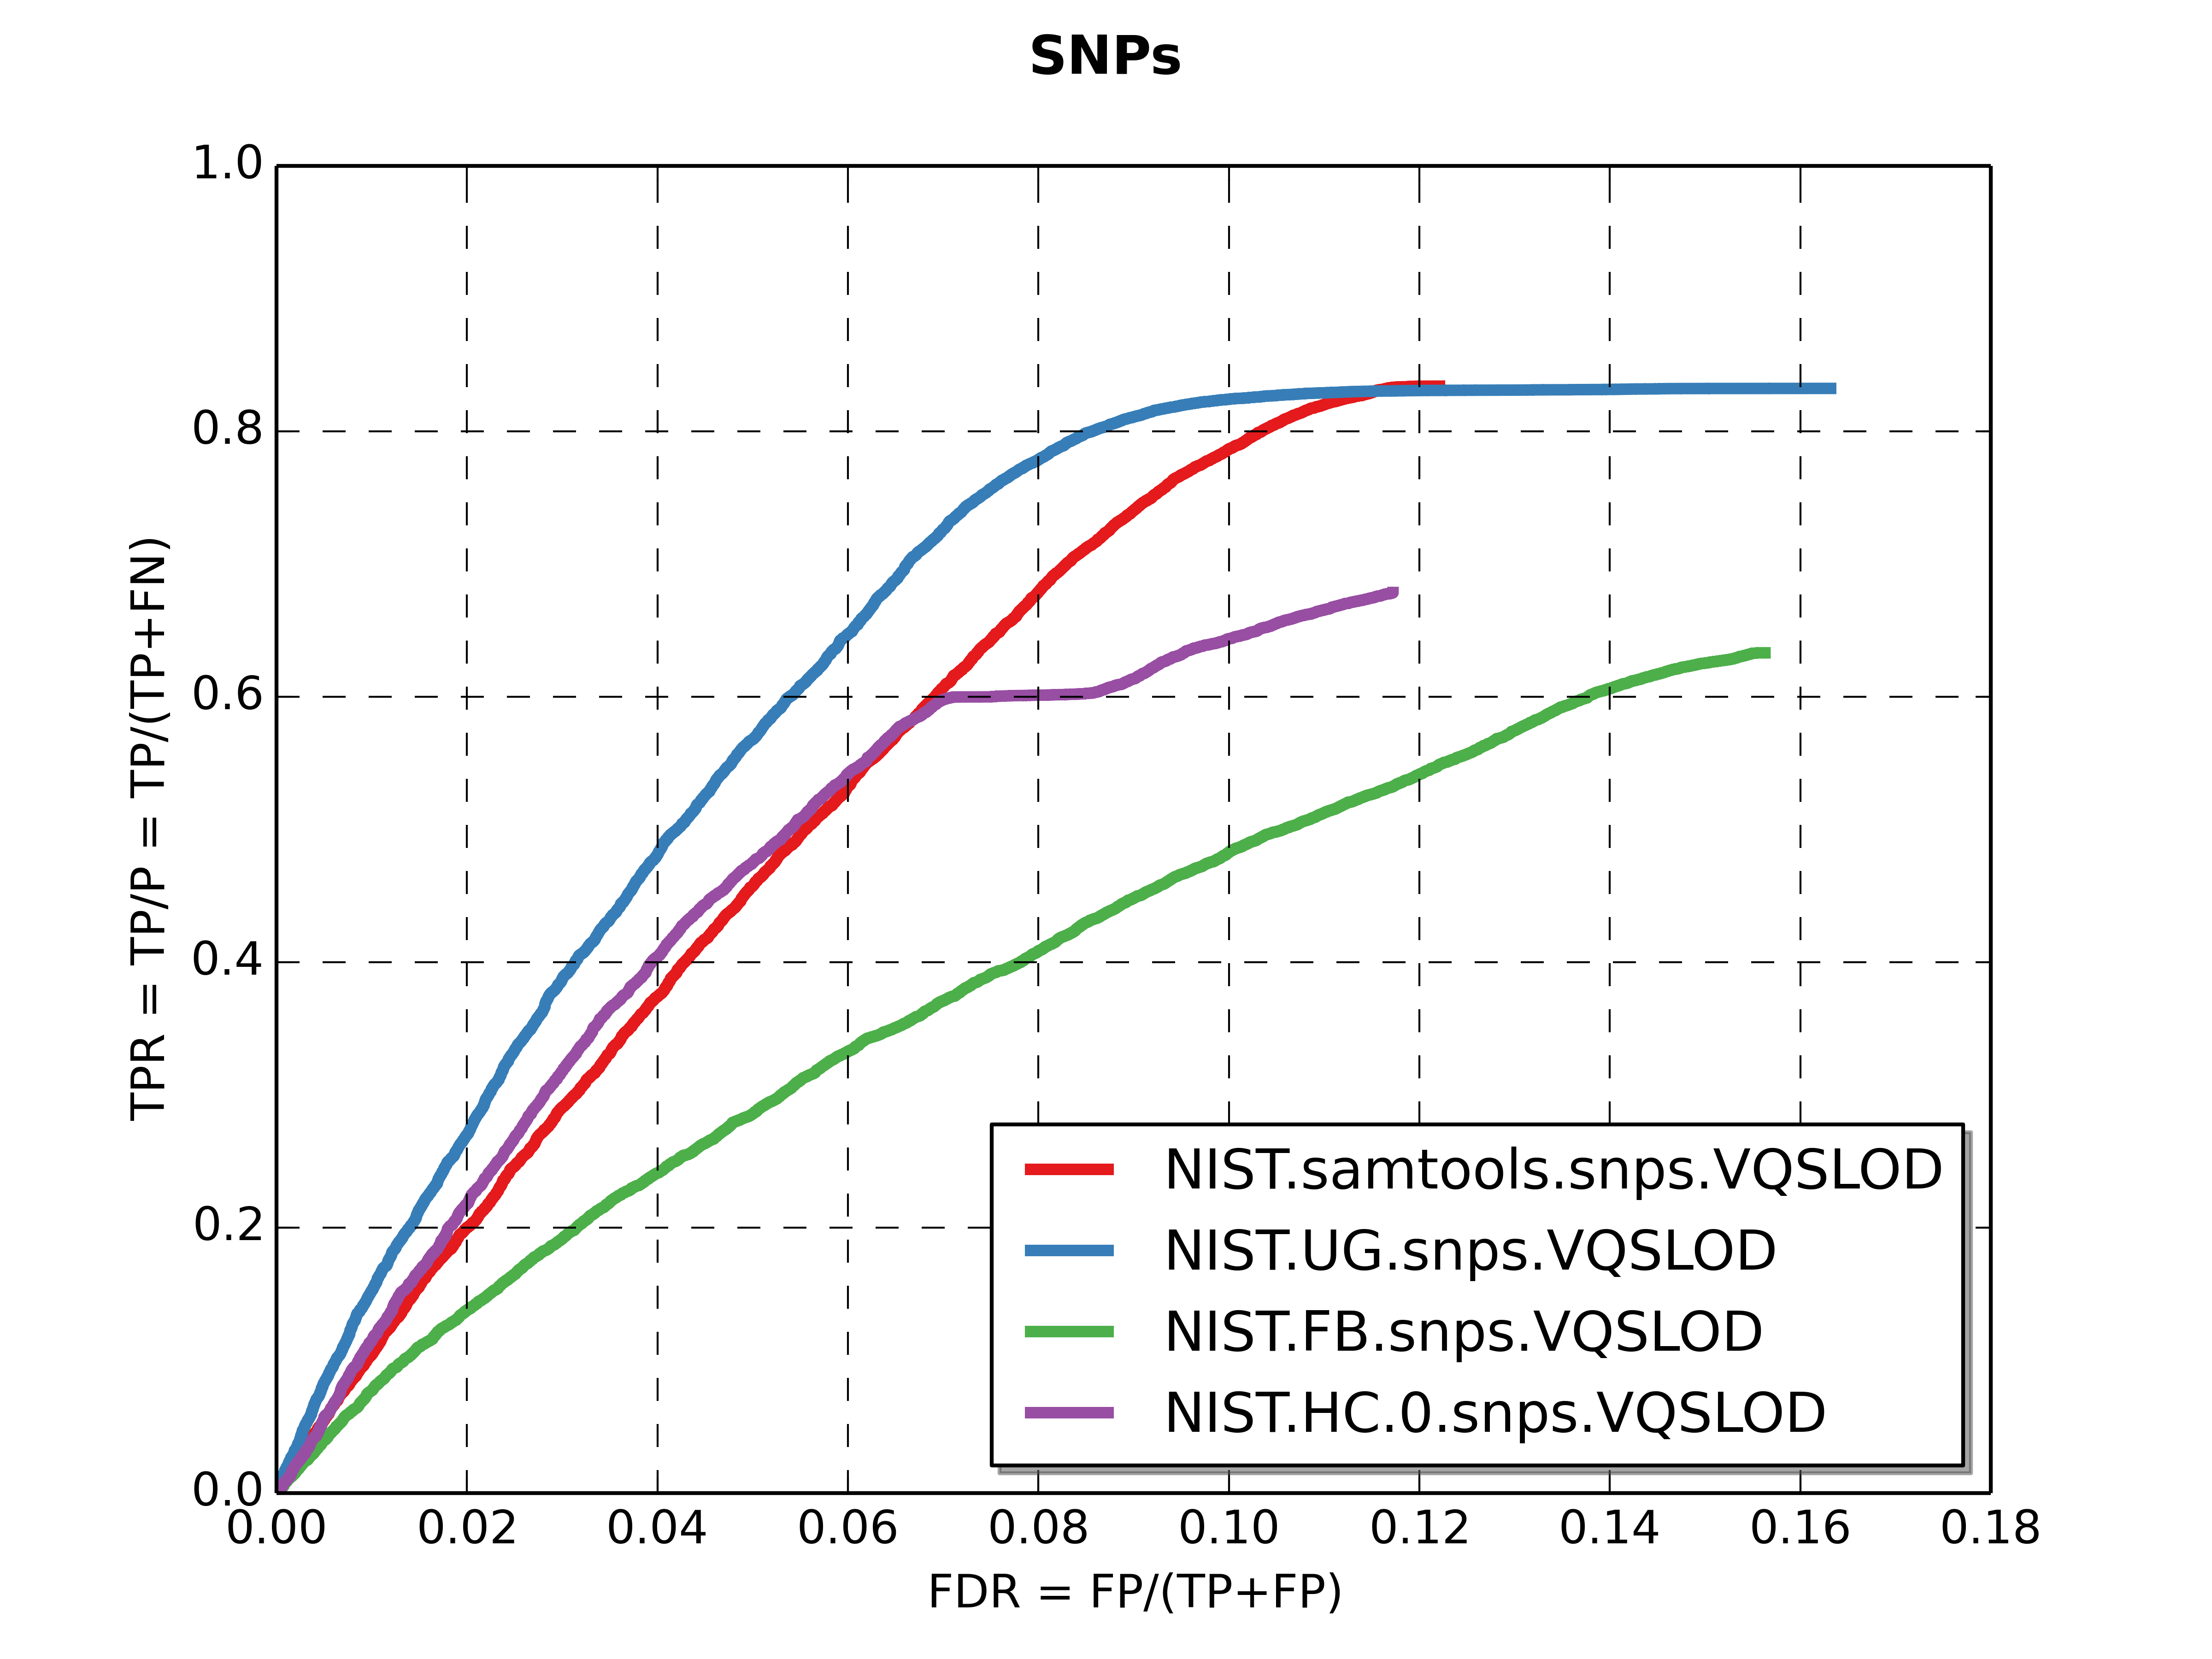
\includegraphics[width=\textwidth]{FDR_snps}
%        \caption{SNPs}
%        \label{fig:roc_snps}
%    \end{subfigure}%
%    \begin{subfigure}[b]{0.45\textwidth}
%        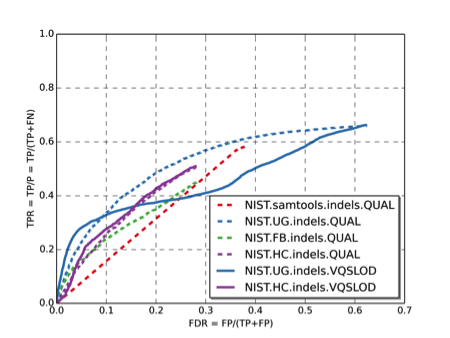
\includegraphics[width=\textwidth]{FDR_indels}
%        \caption{Indels}
%        \label{fig:roc_indels}
%    \end{subfigure}%
\end{figure}

%For high coverage data, we evaluated the NA12878 sample alone re-sequenced on the X-10 pipeline with the highly curated set of variants produced by GiaB.1 We showed that the X-10 and the new pipeline used with it produced high quality data that when normalised showed a high degree of sensitivity versus the GiaB reference set and a low false discovery rate (Table \ref{table:FDRhigh}). When the Illumina 50x Platinum set, sequenced on the Illumina Hiseq 2000 platform was reprocessed through the same pipeline it produced similarly high results, though the INDEL sensitivity and false discovery rate were slightly better. We believe this may be because of the higher coverage and PCR free library preparation used in the creation of this sequence.

%\begin{table}[h]
\centering
%\resizebox{\textwidth}{!}{%
\begin{tabular}{l|lrrrrr}
\rowcolor[HTML]{333333} 
{\color[HTML]{FFFFFF} Sample} & {\color[HTML]{FFFFFF} Type} & {\color[HTML]{FFFFFF} TP} & {\color[HTML]{FFFFFF} FP} & {\color[HTML]{FFFFFF} FN} & {\color[HTML]{FFFFFF} Sensitivity} & {\color[HTML]{FFFFFF} FDR} \\
 & \cellcolor[HTML]{C0C0C0}SNP & \cellcolor[HTML]{C0C0C0}2914294 & \cellcolor[HTML]{C0C0C0}28213 & \cellcolor[HTML]{C0C0C0}10266 & \cellcolor[HTML]{C0C0C0}0.9965 & \cellcolor[HTML]{C0C0C0}0.0096 \\
\multirow{-2}{*}{Replicate 1} & INDEL & 413639 & 23145 & 34743 & 0.9255 & 0.0530 \\
 & \cellcolor[HTML]{C0C0C0}SNP & \cellcolor[HTML]{C0C0C0}2908260 & \cellcolor[HTML]{C0C0C0}26311 & \cellcolor[HTML]{C0C0C0}14452 & \cellcolor[HTML]{C0C0C0}0.9951 & \cellcolor[HTML]{C0C0C0}0.0090 \\
\multirow{-2}{*}{Replicate 2} & INDEL & 393431 & 24110 & 52542 & 0.8822 & 0.0577 \\
 & \cellcolor[HTML]{C0C0C0}SNP & \cellcolor[HTML]{C0C0C0}2917290 & \cellcolor[HTML]{C0C0C0}21400 & \cellcolor[HTML]{C0C0C0}9844 & \cellcolor[HTML]{C0C0C0}0.9966 & \cellcolor[HTML]{C0C0C0}0.0073 \\
\multirow{-2}{*}{Platinum} & INDEL & 437875 & 8802 & 2297 & 0.9948 & 0.0197
\end{tabular}
%}
\caption{Intersect of NA12878 samples with GiaB reference calls version 0.2.}
\label{table:FDRhigh}
\end{table}